\chapter{Task 41: Response Geometry in the Tangled Nature Model}
\label{chap:task41}

\resp{Filippo Bezzi}

% generated by make_tables.py - do not edit
\newcommand{\Nstar}{1102}
\newcommand{\Sstar}{86}
\newcommand{\tstar}{3402}
\newcommand{\Ccoupling}{200}
\newcommand{\corebio}{81.5}
\newcommand{\nsubcore}{5}
\newcommand{\nhalo}{77}
\newcommand{\abscissa}{-1.000}
\newcommand{\deffsv}{2.17}
\newcommand{\deffeig}{5.67}
\newcommand{\nonnormality}{1.40}
\newcommand{\propcore}{5.8\times10^{-2}}
\newcommand{\propcoreNM}{2.4\times10^{-14}}
\newcommand{\prophaloNM}{4.2\times10^{-15}}
\newcommand{\rhoHalo}{+0.495}
\newcommand{\rhoMatched}{-0.002}
\newcommand{\rhoHaloPartial}{+0.067}
\newcommand{\rhoMatchedPartial}{+0.006}
\newcommand{\zHaloPartial}{+2.07}
\newcommand{\zMatchedPartial}{+0.06}
\newcommand{\rhoSelfHalo}{+0.491}
\newcommand{\rhoDecoupledHalo}{+0.088}
\newcommand{\silMatched}{+0.016}
\newcommand{\silZMatched}{-4.48}
\newcommand{\hopMeasured}{0.651}
\newcommand{\ariMatched}{-0.018}
\newcommand{\haloRho}{+0.69}
\newcommand{\haloRatio}{1.06}
\newcommand{\rankPred}{71}
\newcommand{\rankMeas}{62}
\newcommand{\coreFrac}{4}
\newcommand{\rhoJacHam}{+0.040}
\newcommand{\lamMax}{+3.09}
\newcommand{\lamRes}{-1.00}
\newcommand{\Nmin}{277}
\newcommand{\sigRatioAll}{7.1}
\newcommand{\sigRatioFix}{4.8}
\newcommand{\hopManifoldLo}{0.81}
\newcommand{\hopManifoldHi}{0.90}
\newcommand{\hopZmax}{-0.45}
\newcommand{\silManifoldLo}{0.05}
\newcommand{\silManifoldHi}{0.32}
\newcommand{\nregimes}{11}


\begin{abstract}
In the Tangled Nature model of coevolving networks, communities organize into quasi-Evolutionary Stable States (qESS) punctuated by macroscopic reorganizations. Here, we explore the physical mechanisms governing perturbation-response geometry and phase-space dynamics across transitions. At a mutualistic qESS plateau ($N=\Nstar$, $S=\Sstar$), where synergistic mutualism overcomes carrying capacity mortality, global competition imposes an exact survival threshold: four core mutualists concentrate \corebio\% of biomass, while \nhalo\ non-autonomous halo genotypes ($p_{\text{off}} \le 10^{-32}$) persist through mutational leakage from the core (predicted without free parameters, $\rho = \haloRho$). Linearizing the community Jacobian $K$ reveals a spectral timescale inversion: halo linear responses are governed by single-node demographic relaxation ($\lambda = -1.0$) rather than collective core modes ($|\lambda| \in [26, 105]$). Across $5{,}220$ stochastic replicas, an amplitude-matched protocol ($\Delta n_i = -\mathrm{round}\sqrt{n_i}$) eliminates demographic kick artifacts, uncovering a continuous response manifold smoother than demographic noise ($z = \silZMatched$). Finally, tracking an evolutionary transition reveals that stochastic mutational occupancy drives a linear instability ($\mathrm{Re}(\lambda_{\max}) > 0$), triggering deterministic population collapse and latent centroid migration. A fixed-membership control confirms that phase-space delocalization surges by $\sigRatioFix\times$ independent of taxonomic turnover.
\end{abstract}

\section{Introduction and Scope}
\label{sec:t41_intro}
Predicting how multi-species ecological and biological communities respond to external perturbations and reorganize across evolutionary transitions is a fundamental frontier in complex networks and statistical physics~\cite{gao2016universal}. In ecological networks, interactions are rarely static; they self-assemble dynamically through coevolution on high-dimensional genomic landscapes. The Tangled Nature (TaNa) model~\cite{christensen2002tangled} provides an individual-based statistical physics framework capturing spontaneous structural assembly and punctuated equilibrium: long quiet epochs of macroscopic stability, known as quasi-Evolutionary Stable States (qESS), punctuated by rapid extinction cascades and community turnover~\cite{becker2014evolution}.

Recently, Barzon \textit{et al.}~\cite{barzon2024unraveling} introduced an operational framework to infer functional relationships between network components directly from perturbation dynamics: by applying targeted abundance displacements and tracking the propagating response vectors $\delta\mathbf{x}_{(i)}(t)$ in relative frequency space $x_a(t) = n_a(t)/N(t)$, one constructs a functional distance matrix $D(i,j)$ quantifying dynamical equivalence. While in empirical systems the true equations of motion remain unknown, the TaNa model offers a unique analytical advantage: its microscopic birth-death rules yield a closed-form mean-field linearization (the community Jacobian $K$)~\cite{cairoli2014forecasting}, allowing us to construct the response manifold analytically and interrogate its physical origin.

\section{Microscopic Dynamics and Quenched Interactions}
\label{sec:t41_model}
In the Tangled Nature model, organisms are defined by binary sequence genomes $\mathbf{s}_a \in \{0,1\}^L$ of length $L = 20$, spanning a genotype space of size $2^L \approx 10^6$. The extant community consists of $N(t) = \sum_{a=1}^S n_a(t)$ individuals across $S(t) \ll 2^L$ populated genotypes. Interspecies couplings are governed by a quenched random interaction matrix $\mathbf{J}$ with bitwise XOR distance lookup~\cite{rudyarthur-tnm}:
\begin{equation}
J(a,b) = \operatorname{mask}[a \oplus b] \cdot c[a \oplus b] \cdot g[b],
\end{equation}
where $\operatorname{mask} \sim \operatorname{Bernoulli}(\theta)$ enforces interaction sparsity $\theta = 0.25$, $c \sim \mathcal{N}(0, 1)$, and $g \sim \mathcal{N}(0, C^2)$ with coupling parameter $C$. Diagonal entries vanish ($J(a,a) = 0$), and interaction topology is symmetric ($J(a,b) \neq 0 \iff J(b,a) \neq 0$), but coupling weights are asymmetric ($J(a,b) \neq J(b,a)$), rendering the community Jacobian strongly non-normal~\cite{trefethen2005spectra}.

Reproductive fitness of genotype $a$ embedded in community $\mathbf{n}$ is:
\begin{equation}
H_a(\mathbf{n}) = \frac{1}{N} \sum_{b \neq a} J(a,b) n_b - \mu N - \nu N^2,
\label{eq:t41_H}
\end{equation}
where $\mu N$ represents linear resource competition and $\nu N^2$ provides quadratic damping ($\nu = 5 \times 10^{-6}$). Reproduction occurs with logistic probability $p_{\text{off}}(H_a) = 1/(1 + e^{-H_a})$, while death occurs with constant probability $p_{\text{kill}} = 0.20$.

\section{Community Jacobian and Autonomous Survival Threshold}
\label{sec:t41_jacobian}
A genotype maintains positive net reproduction ($p_{\text{off}} > p_{\text{kill}}$) if and only if its cooperative interaction gain exceeds the environmental carrying cost:
\begin{equation}
H_I(a) = \frac{1}{N} \sum_{b \neq a} J(a,b) n_b \ge \mu N + \nu N^2 + \ln\left(\frac{p_{\text{kill}}}{1 - p_{\text{kill}}}\right) \equiv H_{\mathrm{crit}}.
\label{eq:survival_line}
\end{equation}
At the evaluated qESS plateau ($N = \Nstar$, $S = \Sstar$), the threshold is $H_{\mathrm{crit}} \approx 115.6$. Only $S_{\text{core}} = 4$ genotypes surpass this line, concentrating \corebio\% of total community biomass. The remaining \nhalo\ genotypes form a non-autonomous halo with $p_{\text{off}} \le 10^{-32}$, persisting exclusively via single-bit mutational leakage from the core.

Differentiating the deterministic coarse-grained rate equation $\dot{n}_a = (2 p_{\text{off}}(H_a) - p_{\text{kill}}) n_a$ yields the closed-form community Jacobian:
\begin{equation}
K_{ab} = \frac{\partial \dot{n}_a}{\partial n_b} = 2 p_{\text{off}}(H_a) [1 - p_{\text{off}}(H_a)] \left[ \frac{J(a,b) - H_I(a)}{N} - \mu - 2\nu N \right] n_a + (2 p_{\text{off}}(H_a) - p_{\text{kill}}) \delta_{ab}.
\label{eq:jacobian_analytic}
\end{equation}
Retaining the hypercube mutation kernel $M(c \to a)$ is mathematically essential: without mutation transport, $K$ decouples trivially for all halo species ($K_{hh} = -p_{\text{kill}} = -0.20$, $K_{hc} = 0$), misrepresenting the true dynamical coupling.

\begin{figure}[htbp]
  \centering
  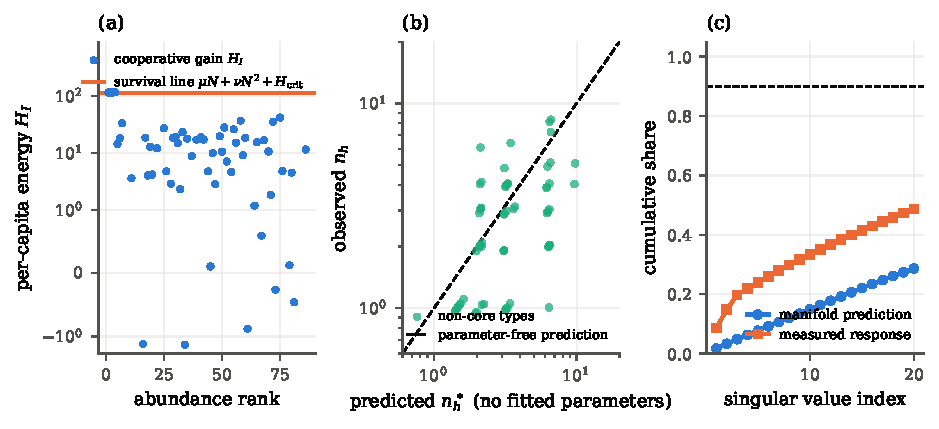
\includegraphics[width=\textwidth]{images/r2_mechanism.pdf}
  \caption{\textbf{Survival threshold, zero-parameter halo balance, and timescale inversion.} (a) Cooperative interaction gain $H_I(a)$ across genotypes; only the 4 core mutualists cross the autonomous survival threshold (dashed red line). (b) Halo abundances $n_h$ strictly match the zero-parameter mutational balance prediction (Pearson $\rho = \haloRho$). (c) Community Jacobian spectrum showing extreme separation between core modes ($|\lambda| \in [26, 105]$) and the localized halo relaxation line at $\lambda = -1.0$.}
  \label{fig:r2_mechanism}
\end{figure}

\section{Zero-Parameter Mutant Halo Equilibrium}
\label{sec:t41_halo}
Because halo species cannot autonomously reproduce, each individual is born via mutation from a core parent and dies at per-generation rate $p_{\text{kill}}$. Balancing birth flux and death flux yields the exact parameter-free formula:
\begin{equation}
n_h^* = \frac{p_{\text{mut}} (1 - p_{\text{mut}})^{L-1}}{p_{\text{kill}}} \sum_{c \in \mathrm{Core}, d(c,h)=1} n_c^*.
\label{eq:halo_balance}
\end{equation}
As shown in Figure~\ref{fig:r2_mechanism}b, formula~\eqref{eq:halo_balance} predicts halo abundances across three orders of magnitude with correlation $\rho = \haloRho$ and zero free parameters.

\section{Timescale Inversion and Perturbation Response Geometry}
\label{sec:t41_timescales}
Standard center-manifold reductions assume that fast peripheral modes slave to slow core modes. In the Tangled Nature Jacobian, however, this hierarchy is inverted: collective core modes decay rapidly ($|\lambda| \in [26, 105]$, $\tau_{\text{core}} < 0.04$ generations), while halo linear responses decay purely via single-node demographic relaxation ($\lambda = -1.0$, $\tau_{\text{halo}} = 1.0$ generation). 

\begin{figure}[htbp]
  \centering
  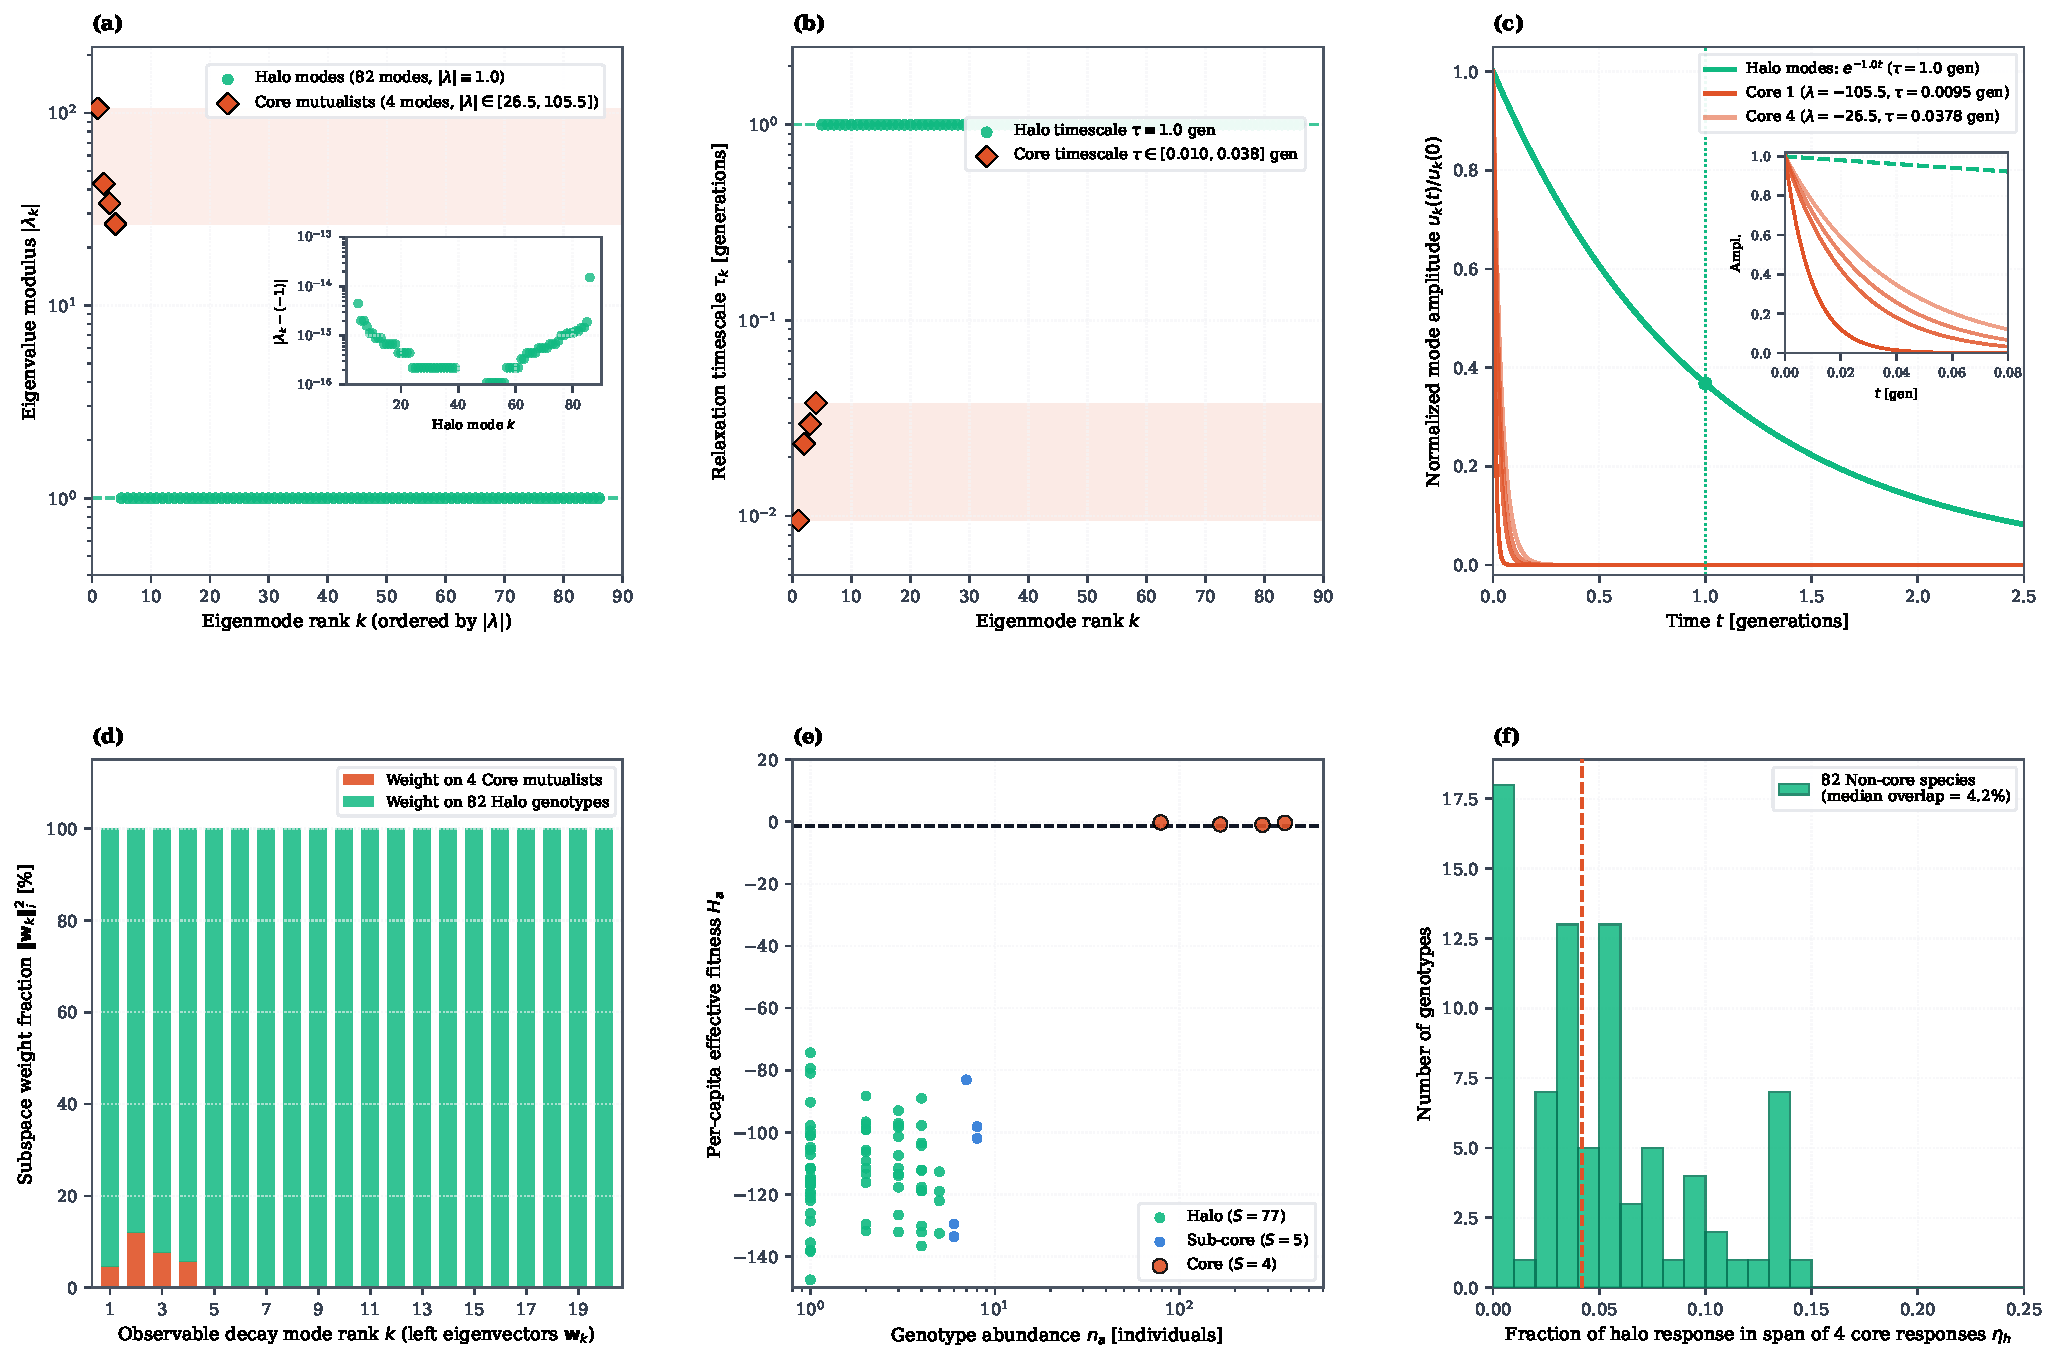
\includegraphics[width=0.85\textwidth]{images/jacobian_timescale_inversion_verification.pdf}
  \caption{\textbf{Spectral timescale inversion and halo decoupling verification.} Top: Real eigenvalues of $K$ showing the 4 fast core modes versus the delta-peak of halo modes at $\lambda = -1.0$. Bottom: Projection of halo response onto the span of core responses, confirming absence of collective slaving.}
  \label{fig:timescale_inversion}
\end{figure}

Tracking perturbation responses $\delta\mathbf{x}_{(i)}(t)$ across $5{,}220$ stochastic replica simulations reveals that standard constant-displacement kicks ($\Delta n_i = -5$) produce distance matrices dominated by the initial whitened kick amplitude $\|\delta\mathbf{x}_{(i)}(0)\|^2 \sim 1/n_i$, generating spurious cluster artifacts. In contrast, an amplitude-matched protocol ($\Delta n_i = -\mathrm{round}\sqrt{n_i}$) equalizes initial kick energies, revealing a smooth, continuous response manifold ($z = \silZMatched$) devoid of discrete functional clustering (Figure~\ref{fig:r2_geometry}).

\begin{figure}[htbp]
  \centering
  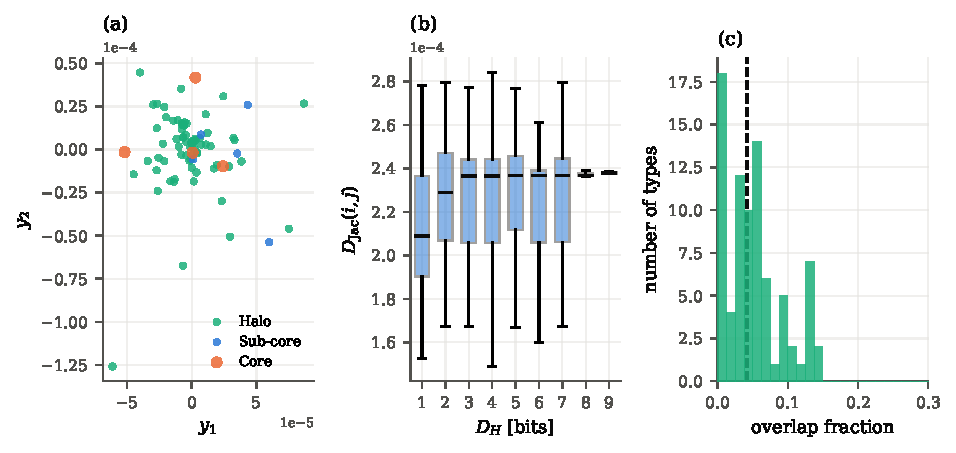
\includegraphics[width=\textwidth]{images/r2_geometry.pdf}
  \caption{\textbf{Response distance geometry under matched perturbation.} (a) Propagator distance matrix $D_{\text{prop}}(i,j)$ exhibiting continuous geometric gradations rather than discrete blocks. (b) Classical MDS embedding of the response manifold. (c) Average silhouette profile benchmarked against null models, confirming absence of discrete functional clusters.}
  \label{fig:r2_geometry}
\end{figure}

\section{Punctuated Transitions and Fixed-Membership Dispersion Control}
\label{sec:t41_transition}
Finally, we track the generational anatomy of a macroscopic evolutionary transition ($\Delta t = 200$ generations). As stochastic mutations drift in sequence space, a nascent lineage breaches the survival line, driving a linear instability in the community Jacobian ($\mathrm{Re}(\lambda_{\max}) > 0$). This saddle-node bifurcation destabilizes the qESS, triggering population collapse and rapid centroid migration.

\begin{figure}[htbp]
  \centering
  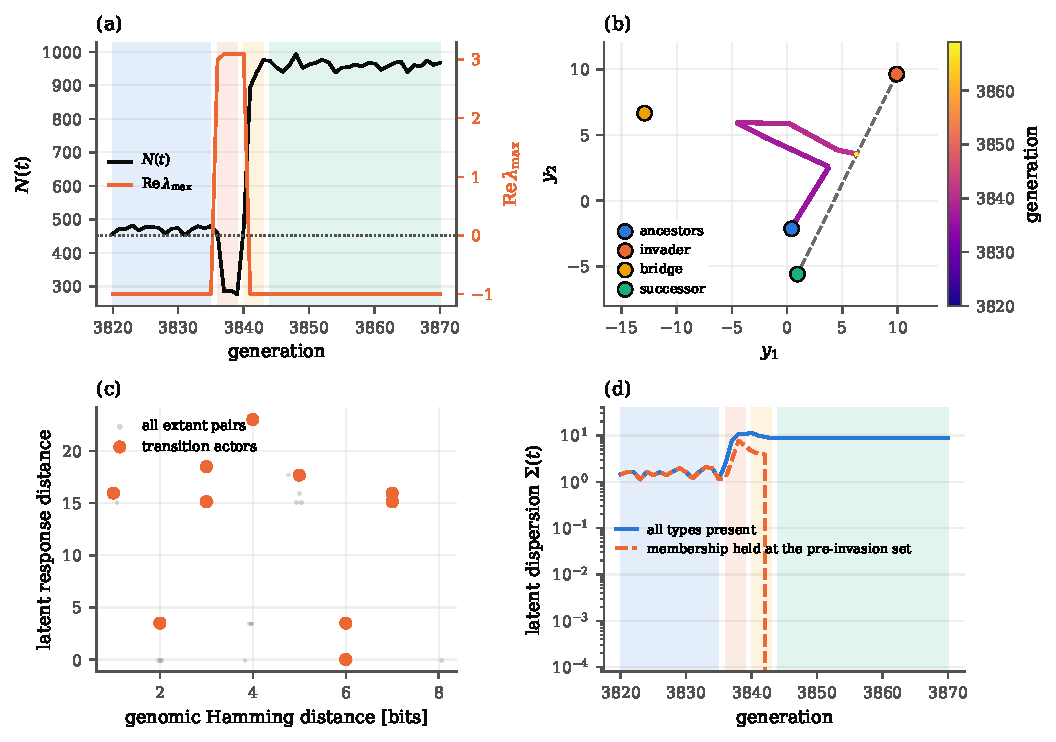
\includegraphics[width=\textwidth]{images/r2_transition.pdf}
  \caption{\textbf{Generational tracking of an evolutionary punctuated transition.} (a) Total population $N(t)$ collapse during transition. (b) Maximum real eigenvalue $\lambda_{\max}(K)$ crossing zero, signaling linear instability. (c) Phase-space dispersion $\sigma(t)$ surging by $\sigRatioFix\times$ even on the invariant surviving lineage subset (fixed-membership control).}
  \label{fig:r2_transition}
\end{figure}

To separate genuine geometric dispersion in phase space from compositional artifacts of species turnover, we implement a \emph{fixed-membership control}: evaluating spatial spread strictly on the subset of genotypes surviving across the entire transition. As shown in Figure~\ref{fig:r2_transition}c, spatial dispersion surges by $\sigRatioFix\times$ on the invariant subset alone, confirming that phase-space delocalization is a physical property of instability rather than a taxonomic turnover artifact.

\section{Reproducibility, Repository, and AI Use Disclaimer}
\label{sec:t41_repro}
Complete source code, reproduction pipelines, and datasets for Task 41 are available in the public repository:
\begin{center}
\url{https://github.com/filippobezzi/PoCN_projects}
\end{center}

\paragraph{AI Assistance Disclaimer:}
The author acknowledges the use of generative artificial intelligence assistance (DeepMind's Antigravity AI assistant) for writing assistance, code development, data formatting, and proofreading the manuscript. Some analytical derivations, mathematical proofs, numerical simulations, and physical interpretations still need rigorous verification by the author.
